
\chapter{Getting started with PETSc}
\label{chap:getstarted}

\section{A code that does almost nothing, but in parallel}

The purpose of the \PETSc library is to help you solve scientific and engineering problems, such as PDEs, on multi-processor computers.  As \PETSc is built ``on top of'' the Message Passing Interface (MPI; \citep{Groppetal1999}) library, some of the MPI flavor comes through.  Therefore we start with an an introductory MPI code which calls \PETSc for some basic tasks.

This code \texttt{c1e.c}, shown in its entirety in Figure \ref{code:e}, approximates Euler's constant
\begin{equation}
e = \sum_{n = 0}^\infty \frac{1}{n!} \approx 2.718281828 \label{introeseries}
\end{equation}
It does the computation in a distributed manner by computing one term of the infinite series on each process.  Thus it computes a better estimate of $e$ when run on more MPI processes. While this is a silly use of \PETSc, it is an easy-to-understand parallel computation.

As with any C source code, \texttt{c1e.c} has a function called \texttt{main()} which takes inputs from the command line, namely \texttt{argc} and \texttt{argv},\sidenote{Here \texttt{argc} is an \texttt{int} holding the argument count and \texttt{argv} is an array of strings (i.e.~type \texttt{char**}) holding the command line including all arguments.  However, in all codes in this book we simply pass these arguments on to \PETSc through the \texttt{PetscInitialize()} method.  \PETSc extracts options through this mechanism.} and which outputs an \texttt{int}.  The output is $0$ if the program succeeds.  Also like all C codes, we include needed headers.  Only \texttt{petsc.h} is needed.

The substance of \texttt{c1e.c} is to declare some variables, do a computation on each process, and communicate the results between processes to get an estimate of $e$.

Before we can compile and run \texttt{c1e.c}, \PETSc must be installed.  If it is not already available, go to
\begin{quote}
\href{http://www.mcs.anl.gov/petsc/download/index.html}{\texttt{www.mcs.anl.gov/petsc/download/}}
\end{quote}
to download the source code, and then follow the instructions at
\begin{quote}
\href{http://www.mcs.anl.gov/petsc/documentation/installation.html}{\texttt{www.mcs.anl.gov/petsc/documentation/installation.html}}
\end{quote}
to install.  Be sure to run ``\texttt{make test}'' and see it pass the tests.  If \PETSc is correctly installed then  environment variables \texttt{PETSC\_DIR} and \texttt{PETSC\_ARCH} point to a valid installation, and the MPI command \texttt{mpiexec} is from the same MPI installation as was used in configuring \PETSc.\sidenote{Type ``\texttt{which mpiexec}'' to find which one you are running.  You may need to modify your \texttt{PATH} environment variable to get the right \texttt{mpiexec}.}

Do the following to compile \texttt{c1e.c}:
\begin{cline}
$ cd p4pdes/c/
$ make c1e
\end{cline}
%$
Calling ``\texttt{make}'' uses \texttt{p4pdes/c/makefile}.  An extract of this makefile is shown in Figure \ref{code:c1emakefile}.  For all the codes in this book, the makefile has this form, as recommended in the \PETSc \emph{User's Manual} \citep{petsc-user-ref}.

\inputwhole{../c/c1e.c}{\texttt{p4pdes/c/c1e.c}}{Compute $e$ in parallel with \PETSc.}{code:e}

Run the code like this:
\begin{cline}
$ ./c1e
e is about 1.000000000000000
rank 0 did 1 flops
\end{cline}
%$
The value $1.0$ is a very poor estimate of $e$, but this code does better with more MPI processes:
\begin{cline}
$ mpiexec -n 5 ./c1e
e is about 2.708333333333333
rank 0 did 0 flops
rank 4 did 3 flops
rank 2 did 1 flops
rank 3 did 2 flops
rank 1 did 0 flops
\end{cline}
%$
That's a better estimate of $e$, but hardly impressive.  On the other hand, with $N=20$ processes, and thus $N=20$ terms in series \eqref{introeseries}, we get a good estimate:
\begin{cline}
$ mpiexec -n 20 ./c1e
e is about 2.718281828459045
rank 0 did 0 flops
...
\end{cline}
%$

\cinputraw{c1emakefile.frag}{extract from \texttt{p4pdes/c/makefile}}{All \texttt{makefile}s for our \PETSc codes look like this.}{}{//START}{//STOP}{code:c1emakefile}

Perhaps the reader is now worried that this book was written using a large supercomputer whereas the reader has a little laptop with only a couple of cores.  In fact these five or twenty process runs work just fine on the author's laptop.  MPI processes are created as needed, using an old feature of operating systems: multitasking.  Speedup from parallelism is another matter; we will return to it.

The main job in \texttt{c1e.c} is to collect the sum of the terms of series \eqref{introeseries} onto each process.  Each process computes term $1/n!$, where $n$ is returned by \texttt{MPI\_Comm\_rank()}.  More precisely, \texttt{PETSC\_COMM\_WORLD} is an MPI communicator \citep{Groppetal1999} containing all processes generated by \texttt{mpiexec} in the above calls, and $n$ is the rank of the process in this communicator.  Then a call to \texttt{MPI\_Allreduce()} does the sum and then sends it back to each process.  These direct uses of the MPI library are a part of using \PETSc because \PETSc generally avoids duplicating MPI functionality.

We print the computed estimate of $e$, but each process also prints its rank and the work it did.  The formatted print command \texttt{PetscPrintf()}, which is like \texttt{fprintf()} from the C standard library, is called twice, once with MPI communicator \texttt{PETSC\_COMM\_WORLD} and once with \texttt{PETSC\_COMM\_SELF}.  The first of these printing jobs is \emph{collective} over all processes, and thus only done once, while the second is individual to each rank.\sidenote{A process is often just called a \emph{rank} in MPI language.}  In the output the \texttt{PETSC\_COMM\_SELF} printed lines can appear in random order because the print occurs as soon as that process reaches that line.

Every \PETSc program should start and end with the commands \texttt{PetscInitialize()} and \texttt{PetscFinalize()}:
\begin{code}
PetscInitialize(&argc,&args,(char*)0,help);
... everything else goes here ...
PetscFinalize();
\end{code}
As an argument to \texttt{PetscInitialize()} we supply a \texttt{help} string.  This string is a good place to say what is the purpose of the code.  To see the help string, and a longer list of possible \PETSc options, do:
\begin{cline}
$ ./c1e -help
\end{cline}
%$
or
\begin{cline}
$ ./c1e -help | less
\end{cline}
%$
Through \texttt{-help}, \PETSc programs have a built-in help system for runtime options that is both light-weight and surprisingly-effective.  For example, to see options related to logging performance, do
\begin{cline}
$ ./c1e -help | grep log_
\end{cline}
%$
We will see later how to add options to our own programs so that they will be documented in the same way.

Unfortunately, \texttt{c1e.c} and all other \PETSc programs have error-checking clutter.  While languages other than C might help with decluttering, we are stuck with ugly lines that look like
\begin{code}
ierr = PetscCommand(...); CHKERRQ(ierr);
\end{code}
The explanation is that almost all \PETSc methods, and most user-written methods in \PETSc programs, return an \texttt{int} for error checking, with value $0$ if successful.  In the line above, \texttt{ierr} is passed to the \texttt{CHKERRQ()} macro which does nothing if \texttt{ierr == 0} but which stops the program with a ``traceback'' otherwise.\sidenote{A traceback is a list of the nested methods, in reverse order, showing the line numbers and method names of the location where the error occurred.}  This traceback mechanishm tends to be the first line of defense when debugging run-time errors.  It is most effective if \PETSc is configured with debugging symbols, i.e.~with the option \texttt{--with-debugging=1}.

Examples in this book always capture-and-check the returned error code using \texttt{ierr} and \texttt{CHKERRQ()}; these are always present in the \texttt{.c} sources in \texttt{p4pde/c/}.  However, after this chapter we will strip the ``\texttt{ierr =}'' and ``\texttt{CHKERRQ(ierr);}'' clutter from the code displayed in the text.


\section{Linear systems}

Our goal is to compute more interesting quantities than Euler's constant $e$.  At the core of most \PETSc computations is a finite-dimensional linear system.  Before solving such systems in \PETSc, we recall the most basic ideas of numerical linear algebra.

Suppose $\bb\in \RR^{N}$ is a column vector and $A\in\RR^{N\times N}$ is a square matrix.  The linear system
\begin{equation}
A \bu = \bb \label{introsystem}
\end{equation}
has a unique solution if $A$ is invertible, namely
\begin{equation}
\bu = A^{-1} \bb. \label{introsolution}
\end{equation}
This is simple in theory.

It is not so simple in practice, however, to solve large systems on a computer.  There are two key facts to keep in mind while working numerically  \citep{TrefethenBau}:
\renewcommand{\labelenumi}{\roman{enumi})}
\begin{enumerate}
\item \label{limittoaccuracy} \emph{limit to accuracy}:  If real numbers are represented on the computer with machine precision $\eps$ then the solution of \eqref{introsystem} can only be computed within an error $\kappa(A) \eps$ where $\kappa(A) = \|A\|_2 \|A^{-1}\|_2$ is the (2-norm) \emph{condition number} of $A$.
\item \emph{cost of direct solutions}:  Computation of solution \eqref{introsolution} by a direct method like Gauss elimination,\sidenote{Or by QR, so that we have a \emph{backward stable} direct method.} whether actually forming $A^{-1}$ or not, is an $O(N^3)$ operation.
\end{enumerate}

Fact i) is about \emph{conditioning} not \emph{methods}.  Informally speaking, there are linear systems that are the same to within $\eps$ but for which the infinite-precision solutions $\bu$ differ by an amount $\kappa(A) \eps$.

On modern computers the precision for the C \texttt{double} type, the default 64-bit representation of real numbers, is $\eps = 2.2 \times 10^{-16}$.  Thus by i), a linear system having $\kappa(A) \approx 10^{10}$, for example, can only be solved to about six digits of precision.  While a matrix with such a large condition number is ``poorly-conditioned,'' it is easy to reach that level for $\kappa(A)$ when discretizing PDEs.  We have to be aware of conditioning when forming expectations about solution accuracy.

By ii) a generic linear system with $N=10^6$ equations requires $10^{18}$ or so operations to solve by Gauss elimination.  Even modern supercomputers take a while to do a quintillion operations.  However, though Gauss elimination is impractical for systems of $N=10^6$ equations, we will successfully solve PDE-generated linear systems of this size on a single processor in a few seconds, and in $O(N)$ operations, in Chapter \ref{chap:multigrid}.  The key fact that discretized PDEs generate linear systems with exploitable structure, especially \emph{sparsity} but also coefficient smoothness, will have to be exposed in serious numerical PDE solutions because naive application of direct methods is too slow.
%time ./c4poisson -da_refine 7 -ksp_type cg -pc_type mg
%on 1153 x 1153 grid:  iterations 2, residual norm = 1.88082e-05
%real 11.18


\section{\PETSc \pVec and \pMat objects}

To build our first \PETSc code to solve a linear system, we need the \PETSc \emph{objects} which store vectors (\pVec) and matrices (\pMat).  Note that, although \PETSc is written in C and not C++, it is a relentlessly object-oriented software library.  Consider the operations which could create and configure a matrix object \texttt{A} for linear system \eqref{introsystem}:
\begin{code}
Mat A;
MatCreate(COMM,&A);
MatSetSizes(A,PETSC_DECIDE,PETSC_DECIDE,N,N);
PetscObjectSetName((PetscObject)A,"A");
MatSetOptionsPrefix(A,"a_");
MatSetFromOptions(A);
... fill entries of (i.e. assemble) A ...
... solve system with A ...
MatDestroy(&A);
\end{code}
We can think of these calls as using methods ``owned'' by the \pMat type, in the sense that these methods manipulate the internal representation of a \pMat while we are (happily) unaware of those details.  At least a \pMat is an \emph{abstract data type} with a hidden implementation.

Even the act of filling entries will treat a \pMat as an abstract object.  Furthermore the data structure inside depends on runtime choices, the most basic being that the number of bytes used to store entries on a given MPI process will depend on the number of processes.  Actually a \PETSc \pMat object need not even have entries.  It might, instead, contain code that applies a linear operator to vectors.

For all \PETSc object types this basic sequence of operations applies:
\begin{code}
Object X;
ObjectCreate(COMM,&X);
... code sets properties of X ...
ObjectSetFromOptions(X);  // allows run-time setting
                          // or overriding of properties
... code uses X ...
ObjectDestroy(&X);
\end{code}
(Here ``\texttt{Object}'' is a meta-name for a \PETSc type like \pVec or \pMat.)

Because \PETSc objects are generally distributed across, and accessible from, multiple MPI processes., the first argument of an \texttt{ObjectCreate()} method is an MPI communicator (``\texttt{COMM}'').  All processes in \texttt{COMM} must call the \texttt{ObjectCreate()} and  \texttt{ObjectDestroy()} methods.

In the \pMat code above, note the call to \texttt{MatSetOptionsPrefix()}.  Through this ``prefix'', run-time options can address the particular \pMat object.  For example, the run-time option \texttt{-a\_mat\_view} will print out the entries of \texttt{A}.  An option prefix like ``\texttt{a\_}'' is especially helpful in distinguishing multiple \pMat objects at the command line.

Once \pMat \texttt{A} is created and set up by the first five commands \texttt{MatCreate()}--\texttt{MatSetFromOptions()}, then various methods become valid for \texttt{A}, for example including the \texttt{MatSetValues()} method to set entries in \texttt{A}.  We will use that method soon.


\section{Assembly and parallel layout of \pVecs and \pMats}

A \pVec or \pMat stores its entries in parallel across all the processes in the MPI communicator used when creating it.  For example, the create-assemble sequence of a \pVec with four entries might look like
\begin{code}
Vec x;
PetscInt   i[4] = {0, 1, 2, 3};
PetscReal  v[4] = {11.0, 7.0, 5.0, 3.0};

VecCreate(COMM,&x);
VecSetSizes(x,PETSC_DECIDE,4);
VecSetFromOptions(x);
VecSetValues(x,4,i,v,INSERT_VALUES);
VecAssemblyBegin(x);
VecAssemblyEnd(x);
\end{code}
The four entries of \texttt{Vec x} are set by \texttt{VecSetValues()}, putting values from array \texttt{v} at the indices given by \texttt{i}.

Potentially the operation of setting values in \texttt{x} requires communication between processes, because entries of \texttt{x} which are to be stored on one process could be set by another process.  Such communication occurs between the \texttt{VecAssemblyBegin()} and \texttt{VecAssemblyEnd()} commands.

\begin{marginfigure}
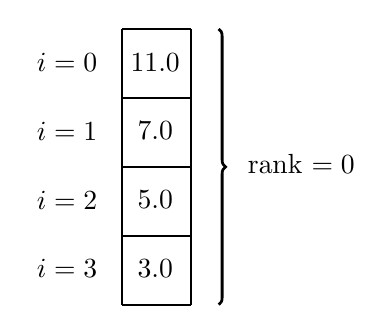
\begin{tikzpicture}[scale=3.5]
  \pgfmathsetmacro\fourth{1.0/4.0}
  \pgfmathsetmacro\xoff{0.12}
  \pgfmathsetmacro\yoff{0.12}
  \draw[xstep=\fourth,ystep=\fourth,black,thick] (0.0,0.0) grid (\fourth,1.0);
  \node at (-0.2,1.0-\yoff) {$i=0$};
  \node at (\xoff,1.0-\yoff) {$11.0$};
  \node at (-0.2,0.75-\yoff) {$i=1$};
  \node at (\xoff,0.75-\yoff) {$7.0$};
  \node at (-0.2,0.5-\yoff) {$i=2$};
  \node at (\xoff,0.5-\yoff) {$5.0$};
  \node at (-0.2,0.25-\yoff) {$i=3$};
  \node at (\xoff,0.25-\yoff) {$3.0$};
  \draw[decoration={brace,mirror,raise=5pt},decorate,line width=1pt] (0.3,0.0) -- (0.3,1.0);
  \node at (0.65,0.51) {rank $=0$};
\end{tikzpicture}
\bigskip
\caption{A sequential \pVec layout, all on rank $=0$ process.}
\label{fig:seqveclayout}
\end{marginfigure}

The reader is allowed to think of a \PETSc \pVec as a one-dimensional C array with its contents split across the processes in the MPI communicator used in the \texttt{VecCreate()} command.  For example, if the above code appears in \texttt{mycode.c}, and if it is run sequentially on one process, i.e.~as
\begin{cline}
$ ./mycode.c
\end{cline}
%$
then, at the end of the above create-set-assemble sequence, the storage of \texttt{x} looks like Figure \ref{fig:seqveclayout}.  However, if run as
\begin{cline}
$ mpiexec -n 2 ./mycode.c
\end{cline}
%$
then the layout looks like Figure \ref{fig:mpitwoveclayout}.  In this case the argument \texttt{PETSC\_DECIDE} in \texttt{VecSetSizes()} is active.  \PETSc decides to put the first two entries of \texttt{x} on the rank $0$ process and the other two on the rank $1$ process. 

\begin{marginfigure}
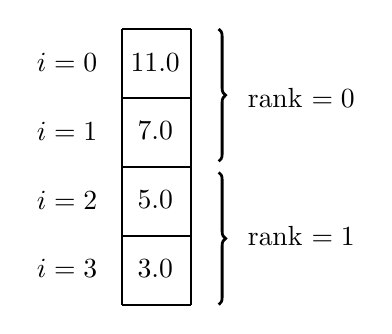
\begin{tikzpicture}[scale=3.5]
  \pgfmathsetmacro\fourth{1.0/4.0}
  \pgfmathsetmacro\xoff{0.12}
  \pgfmathsetmacro\yoff{0.12}
  \draw[xstep=\fourth,ystep=\fourth,black,thick] (0.0,0.0) grid (\fourth,1.0);
  \node at (-0.2,1.0-\yoff) {$i=0$};
  \node at (\xoff,1.0-\yoff) {$11.0$};
  \node at (-0.2,0.75-\yoff) {$i=1$};
  \node at (\xoff,0.75-\yoff) {$7.0$};
  \node at (-0.2,0.5-\yoff) {$i=2$};
  \node at (\xoff,0.5-\yoff) {$5.0$};
  \node at (-0.2,0.25-\yoff) {$i=3$};
  \node at (\xoff,0.25-\yoff) {$3.0$};
  \draw[decoration={brace,mirror,raise=5pt},decorate,line width=1pt] (0.3,0.52) -- (0.3,1.0);
  \node at (0.65,0.752) {rank $=0$};
  \draw[decoration={brace,mirror,raise=5pt},decorate,line width=1pt] (0.3,0.0) -- (0.3,0.48);
  \node at (0.65,0.251) {rank $=1$};
\end{tikzpicture}
\bigskip
\caption{A parallel \pVec layout on two processes.  Because we call ``\texttt{VecSetSizes(x,PETSC\_DECIDE,4)}'', \PETSc decides to split the storage in the middle.}
\label{fig:mpitwoveclayout}
\end{marginfigure}

\pMat objects, however, are not actually 2D C arrays even in serial (i.e.~in one-process runs).  Compared to \pVecs they require additional choices regarding parallel distribution.  Though this is hidden inside the implementation of \pMat, the most common storage format is \emph{parallel compressed sparse row storage}, what \PETSc calls the \texttt{MATMPIAIJ} type.  In this type a range of rows is owned by each process (parallel row storage), and within each owned range of rows only the specifically-allocated\sidenote{These are generally the nonzero entries, and usually referred-to as such.} entries are stored (sparse), and furthermore nonzero entries are stored contiguously in an array using an additional index array (compressed).

\pMat objects are linear operators so their major purpose is to multiply \pVecs.  The result vector of a \pMat-\pVec product is a linear combination of the columns of the \pMat.  Thus, in practice, ``parallel row storage'' of the \pMat means these things:\begin{itemize}
\item \PETSc internally distributes the rows of the \pMat $A$ the same way as the entries of the intended output \pVec.  Thus if $Ax=b$ for some $x$ then the rows of $A$ are distributed like the entries of $b$, at least when \texttt{PETSC\_DECIDE} is used in setting \pVec and \pMat sizes.
\item Before \PETSc computes a \pMat-\pVec product, \PETSc communicates (``scatters'') the whole \pVec to each process.
\item After the scatter the \pMat-\pVec product is a local operation, requiring no further communication.
\end{itemize}

But one doesn't really need to know all this!  For example, here is how to create and assemble a $4\times 4$ \pMat, with essentially random entries, one row at a time:
% see testmatcreate.c
\begin{code}
Mat A;
PetscInt  i, j[4] = {0, 1, 2, 3};
PetscReal v[4];

MatCreate(PETSC_COMM_WORLD,&A);
MatSetSizes(A,PETSC_DECIDE,PETSC_DECIDE,4,4);
MatSetFromOptions(A);
MatSetUp(A);

i = 0;  v[0] = 1.0;  v[1] = 2.0;  v[2] = 3.0;  v[3] = 4.0;
MatSetValues(A,1,&i,4,j,v,INSERT_VALUES);
i = 1;  v[0] = 2.0;  v[1] = 0.0;  v[2] = -2.0;  v[3] = -3.0;
MatSetValues(A,1,&i,4,j,v,INSERT_VALUES);
i = 2;  v[0] = -1.0;  v[1] = 1.0;  v[2] = 1.0;  v[3] = 0.0;
MatSetValues(A,1,&i,4,j,v,INSERT_VALUES);
i = 3;  v[0] = 2.0;  v[1] = 1.0;  v[2] = -1.0;  v[3] = 1.0;
MatSetValues(A,1,&i,4,j,v,INSERT_VALUES);

MatAssemblyBegin(A,MAT_FINAL_ASSEMBLY);
MatAssemblyEnd(A,MAT_FINAL_ASSEMBLY);
\end{code}
The method \texttt{MatSetValues()} sets a \emph{block} of values, in this case a row.  The ``\texttt{1,\&i}'' arguments to \texttt{MatSetValues()} say that we are setting one row with global index \texttt{i}.  The ``\texttt{4,j}'' arguments say that we set the row using integer array \texttt{j} for the (global) column indices.

\begin{marginfigure}
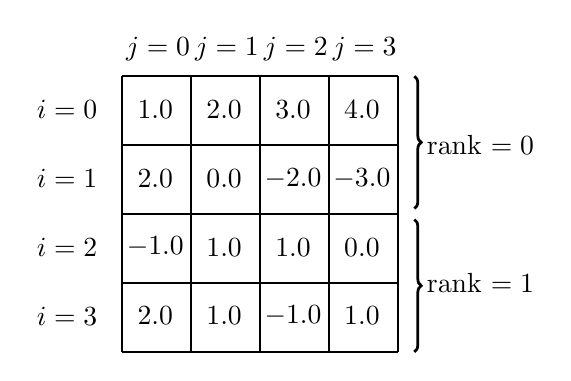
\begin{tikzpicture}[scale=3.5]
  \pgfmathsetmacro\fourth{1.0/4.0}
  \pgfmathsetmacro\xoff{0.12}
  \pgfmathsetmacro\yoff{0.12}
  \draw[xstep=\fourth,ystep=\fourth,black,thick] (0.0,0.0) grid (1.0,1.0);

  \node at (-0.2, 1.0-\yoff) {$i=0$};
  \node at (-0.2,0.75-\yoff) {$i=1$};
  \node at (-0.2, 0.5-\yoff) {$i=2$};
  \node at (-0.2,0.25-\yoff) {$i=3$};

  \node at ( 1.0-\xoff, 1.1) {$j=3$};
  \node at (0.75-\xoff, 1.1) {$j=2$};
  \node at ( 0.5-\xoff, 1.1) {$j=1$};
  \node at (0.25-\xoff, 1.1) {$j=0$};

  \node at (\xoff,1.0-\yoff) {$1.0$};
  \node at (0.25+\xoff,1.0-\yoff) {$2.0$};
  \node at (0.5+\xoff,1.0-\yoff) {$3.0$};
  \node at (0.75+\xoff,1.0-\yoff) {$4.0$};

  \node at (\xoff,0.75-\yoff) {$2.0$};
  \node at (0.25+\xoff,0.75-\yoff) {$0.0$};
  \node at (0.5+\xoff,0.75-\yoff) {$-2.0$};
  \node at (0.75+\xoff,0.75-\yoff) {$-3.0$};

  \node at (\xoff,0.5-\yoff) {$-1.0$};
  \node at (0.25+\xoff,0.5-\yoff) {$1.0$};
  \node at (0.5+\xoff,0.5-\yoff) {$1.0$};
  \node at (0.75+\xoff,0.5-\yoff) {$0.0$};

  \node at (\xoff,0.25-\yoff) {$2.0$};
  \node at (0.25+\xoff,0.25-\yoff) {$1.0$};
  \node at (0.5+\xoff,0.25-\yoff) {$-1.0$};
  \node at (0.75+\xoff,0.25-\yoff) {$1.0$};

  \draw[decoration={brace,mirror,raise=5pt},decorate,line width=1pt] (1.01,0.52) -- (1.01,1.0);
  \node at (1.3,0.752) {rank $=0$};
  \draw[decoration={brace,mirror,raise=5pt},decorate,line width=1pt] (1.01,0.0) -- (1.01,0.48);
  \node at (1.3,0.251) {rank $=1$};
\end{tikzpicture}
\bigskip
\caption{A parallel \pMat layout on two processes.}
\label{fig:mpitwomatlayout}
\end{marginfigure}

If the above lines appeared in \texttt{mycode.c}, and if it was run
\begin{cline}
$ mpiexec -n 2 ./mycode
\end{cline}
%$
then the layout would be as in Figure \ref{fig:mpitwomatlayout}.

We can have \PETSc show us the entries in the \pMat in different formats at the command line:
\begin{cline}
$ ./mycode -mat_view
Mat Object: 1 MPI processes
  type: seqaij
row 0: (0, 1)  (1, 2)  (2, 3)  (3, 4)
row 1: (0, 2)  (1, 0)  (2, -2)  (3, -3)
row 2: (0, -1)  (1, 1)  (2, 1)  (3, 0)
row 3: (0, 2)  (1, 1)  (2, -1)  (3, 1)
$ ./mycode -mat_view ::ascii_dense
Mat Object: 1 MPI processes
  type: seqaij
 1.00000e+00  2.00000e+00  3.00000e+00  4.00000e+00
 2.00000e+00  0.00000e+00  -2.00000e+00  -3.00000e+00
 -1.00000e+00  1.00000e+00  1.00000e+00  0.00000e+00
 2.00000e+00  1.00000e+00  -1.00000e+00  1.00000e+00
\end{cline}
The first view shows the compressed sparse storage, with values as pairs with column index and value.  The second view is a traditional (``dense'') display where all zero values are shown, whether allocated or not.  In these cases the matrix was stored in \emph{serial} compressed sparse row format, the \texttt{MATSEQAIJ} type, because of the one-process execution.

If the code is run in parallel, i.e.~by \texttt{mpiexec -n N ./mycode}, then \texttt{-mat\_view}  reports \texttt{type:~mpiaij} corresponding to \pMat type \texttt{MATMPIAIJ}.  This is the ``parallel compressed sparse row storage'' described above.


\section{A bit more numerical linear algebra}

Direct methods like Gauss elimination \citep{TrefethenBau} are one way to solve a system, but many other methods are iterative.  They are often based on the \emph{residual} of some approximation $\bu_0$ of the solution.  By definition, the residual of $\bu_0$ in linear system \eqref{introsystem} is the vector
\begin{equation}
\br_0 = \bb - A \bu_0. \label{residualdefn}
\end{equation}

Evaluating the residual for a known vector $\bu_0$ requires only applying $A$ to it, an $O(N^2)$ operation at most.  However, most discretization schemes for PDEs generate matrices $A$ that are \emph{sparse}, with many more zero entries than nonzeros, and often the number of nonzeros per row is independent of $N$.  In such cases the operation $A\bu_0$ and the evaluation of the residual can be done in $O(N)$ operations.

The \emph{Richardson iteration} is an example of an iterative method based on the residual.  If $\bu_0$ is an initial estimate of the solution then it simply adds a multiple $\omega$ of the last residual at each step:
\begin{equation}
\bu_{k+1} = \bu_k + \omega (\bb - A \bu_k).  \label{introrichardson}
\end{equation}
If significantly fewer than $O(N^2)$ steps are needed to make $\bu_k$ an adequate approximation of the exact solution $\bu$, then the Richardson iteration can improve on Gauss elimination.  On the other hand, the Richardson iteration may not converge, as in the next Example.

\newcommand{\rvect}[3]{\ensuremath{\bu_{#1} = \begin{bmatrix} #2 \\ #3 \end{bmatrix}}}

\medskip\noindent\hrulefill
\begin{example} Consider the linear system
\begin{equation}
A \bu
= \begin{bmatrix}
10 & -1 \\ -1 & 1
\end{bmatrix}
\begin{bmatrix} u_1 \\ u_2 \end{bmatrix}
= \begin{bmatrix} 8 \\ 1 \end{bmatrix}
= \bb
 \label{introexample}
\end{equation}
which has solution $\bu = [1\,\, 2]^\top$.  If we start with estimate $\bu_0 = [0\,\, 0]^\top$ then the $\omega=1$ Richardson iteration \eqref{introrichardson} gives a sequence of vectors % see ../matlab/richardsonex.m
\begin{equation}
\rvect{0}{0}{0}, \rvect{1}{8}{1}, \rvect{2}{-63}{9}, \rvect{3}{584}{-62}, \dots
\end{equation}
This sequence is not heading toward the solution.
\end{example}
\noindent\hrulefill

\medskip
If we rewrite \eqref{introrichardson} as
\begin{equation}
\bu_{k+1} = (I - \omega A) \bu_k + \omega \bb  \label{introrewriterichardson}
\end{equation}
then it is easy to believe that the ``size'' of the matrix $I-\omega A$ will determine whether $\lim_{k\to\infty} \bu_k$ exists, for generic starting vectors $\bu_0$.  To make this precise we recall the definitions of \emph{eigenvalue} and \emph{singular value}.

A complex number $\lambda \in \CC$ is an eigenvalue of a square matrix $B\in\RR^{N\times N}$ if there is a nonzero vector $\bv\in\CC^N$ so that $B \bv = \lambda \bv$.  The singular values are then the square roots of the eigenvalues of the matrix $B^*B$.  The matrix $B^*B$ is symmetric and positive-definite so its eigenvalues are nonnegative.  Singular values are also geometrically-defined as the lengths of semi-axes of the ellipsoid in $\RR^N$ that results from applying $B$ to all vectors in the unit sphere of $\RR^N$ \citep{TrefethenBau}.

The set of all eigenvalues of $B$ is the \emph{spectrum} $\sigma(B)$ of $B$.  Properties of matrices described in terms of eigenvalues or singular values are generically called ``spectral properties.''  For example, recall that $\|B\|_2$ is equal to the largest singular value of $B$, while $\|B^{-1}\|_2$ is equal to the inverse of the smallest singular value of $B$.  The 2-norm condition number $\kappa(B)$ is the ratio of largest to smallest singular values,\sidenote{The condition number of $B$ is visualized as the eccentricity of the ellipsoid we used in defining the singular values geometrically.} and thus is a spectral property of $B$.

It is an easy exercise to show that the Richardson iteration \eqref{introrichardson} will converge if and only if all the eigenvalues of $B=I-\omega A$ are inside the unit circle.  Defining the \emph{spectral radius} $\rho(B)$ of a matrix $B$ as the maximum norm of the eigenvalues of $A$, we can describe the convergence of the Richardson iteration:
\begin{equation}
\text{\eqref{introrichardson} converges if and only if } \rho(I-\omega A) < 1. \label{introconvergethm}
\end{equation}
One can show that $\rho(B) \le \|B\|_2$, so \eqref{introrewriterichardson} converges if $\|I-\omega A\|_2 < 1$.

The most powerful iterative linear algebra methods generate optimal, in various senses \citep{TrefethenBau}, estimates $\bu_k$ which are each linear combinations of vectors $\bb,A\bb,A^2\bb,\dots,A^{k-1}\bb$.  These methods are collectively called \emph{Krylov space methods} because the span of these vectors is a Krylov space.  Examples are conjugate gradients (CG) and minimum residual methods (e.g.~MINRES or GMRES) \citep{Greenbaum1997}.  (The classical Jacobi and Gauss-Siedel iterative methods are not Krylov space methods because they involve extracting parts of $A$ as a matrix.)  The effectiveness of a given Krylov method on a given matrix $A$ depends on the eigenvalues or singular values of $A$, i.e.~on its spectral properties.  We use Krylov space methods in Chapter \ref{chap:structured} and all later Chapters.

Considering spectral properties brings us to an important general point about linear systems.  Namely, that there are many other systems which are equivalent to \eqref{introsystem}.  In fact, if $P\in\RR^{N\times N}$ is an invertible square matrix then the systems
\begin{equation}
(P^{-1} A) \bu = P^{-1} \bb \label{introleftpre}
\end{equation}
and
\begin{equation}
(A P^{-1}) (P\bu) = \bb \label{introrightpre}
\end{equation}
obviously have the same solution $\bu$ as \eqref{introsystem}.  However, matrices $P^{-1} A$ or $A P^{-1}$ may have different eigenvalues, condition numbers, and so on---different spectral properties---from $A$.  While the accuracy of the approximate solution $\bu$ cannot be improved beyond the $\kappa(A) \eps$ level, as fact i) on page \pageref{limittoaccuracy} cannot be overcome, methods can take advantage of better spectral properties to generate $\bu$ more quickly.  This idea is effective if $P^{-1}$ is easy to apply.\sidenote{This means: the system $P\bv = \bc$ is easy to solve for $\bv$ in the sense of low computational cost.}

Equivalent systems \eqref{introleftpre} and \eqref{introrightpre} are referred to as \emph{preconditioned} systems, with \eqref{introleftpre} called \emph{left preconditioning} and \eqref{introrightpre} called \emph{right-preconditioning}.  The next example shows how preconditioning can make the Richardson iteration converge.

\medskip\noindent\hrulefill
\begin{examplecont}  Suppose we use the diagonal matrix from  \eqref{introexample} as $P$:
\begin{equation}
P = \begin{bmatrix}
10 & 0 \\ 0 & 1
\end{bmatrix}.  \label{introP}
\end{equation}
Being diagonal, this $P$ is easy to invert and apply.  The preconditioned Richardson iteration using $P$, namely
\begin{equation}
\bu_{k+1} = \bu_k + \omega (P^{-1} \bb - P^{-1} A \bu_k),  \label{introprerichardson}
\end{equation}
is better behaved.  With $\bu_0 = [0\,\, 0]^*$ again we get this sequence from \eqref{introprerichardson}:
\begin{equation}
\rvect{0}{0}{0}, \rvect{1}{0.8}{1.0}, \rvect{2}{0.9}{1.8}, \rvect{3}{0.98}{1.90}, \dots
\end{equation}
This sequence is apparently going to $\bu = [1\,\, 2]^*$.  The explanation is not hard to see; compare
\begin{equation}
\rho(I-A) = -9.1, \qquad \rho(I-P^{-1} A) = 0.32.
\end{equation}
This example illustrates convergence claim \eqref{introconvergethm}.
\end{examplecont}
\noindent\hrulefill

\medskip
The above introduction of the residual, Richardson iteration, and preconditioning is hardly adequate.  But let us return to \PETSc codes and solve linear systems.  The reader can first treat \PETSc's linear solver object as a black box, but then explore how it works through runtime options.

\section{Solve a small linear system in \PETSc}

We already know how to create, fill, and destroy \pVec and \pMat objects.  The next code, \texttt{c1vecmatksp.c} shown in Figure \ref{code:vecmatksp}, does these steps.  To solve the system it uses a Krylov space solver object ``\pKSP'' which has the ability to solve a linear system by a method chosen at runtime.

Besides the expected \texttt{Create/SetFromOptions/Destroy} sequence for \pKSP, there are two important commands.  The system is actually solved by
\begin{code}
KSPSolve(ksp,b,x);
\end{code}
This supplies the right-hand side of the system (i.e.~\pVec \texttt{b}) and space for the solution (\pVec \texttt{x}).  But first we tell \pKSP about the matrix in the linear system by the command
\begin{code}
KSPSetOperators(ksp,A,A);
\end{code}

Why list \texttt{A} twice in \texttt{KSPSetOperators}?  As in our brief introduction above, the linear system $A\bx=\bb$ is equivalent to preconditioned systems like $P^{-1} A \bx = P^{-1} \bb$ (for left preconditioning).  At runtime, typically and conceptually, one chooses a preconditioning method which builds $P$ from $A$, or an approximation of $A$, before applying $P^{-1}$.  For example, \emph{incomplete LU} factorization can be used in building $P$ from $A$, or $P$ could be the diagonal of $A$ as in the example.  The second matrix argument supplied to \texttt{KSPSetOperators} is the ``raw data'' from which the preconditioner $P$ is built.  Note we do not \emph{supply} $P$ itself---that would both require the user to write extra code and it would stop the user from choosing among preconditioners at runtime.  Insteady we supply ``material'' from which preconditioner code can build and apply the linear operator $P^{-1}$, and the most common such ``material'' is $A$ itself.

After calling \texttt{KSPSolve()} we view the solution \pVec \texttt{x} by calling \texttt{VecView()}.  But this and everything else about the code in Figure \ref{code:vecmatksp} should be self-explanatory, so now let's run it:
\begin{cline}
$ make c1vecmatksp
$ ./c1vecmatksp
Vec Object: 1 MPI processes
  type: seq
3
4
4
-3
\end{cline}
This solves the system and gives us $\bx$.  But what happened and how to control it?

\inputwhole{../c/c1vecmatksp.c}{\texttt{p4pdes/c/c1vecmatksp.c}}{Solve a small linear system.}{code:vecmatksp}


\section{Revealing actions at runtime}

Now we get to a key \PETSc idea which cannot be over-emphasized:
\begin{quote}
learning \PETSc requires viewing solver objects at runtime.
\end{quote}
For example, what happened in running ``\texttt{./c1vecmatksp}'' above?  Quite a bit!  To start we can view the \pVec and \pMat objects, by ``\texttt{./c1vecmatksp -vec\_view -mat\_view}'' but this tells us nothing about the solver, and gives no hints on changing methods at runtime.  Instead, look at the output of \texttt{-ksp\_view}, here with a bit of the information supressed for brevity:
\begin{cline}
$ ./c1vecmatksp -ksp_view
KSP Object: 1 MPI processes
  type: gmres
    GMRES: restart=30, using Classical (unmodified) Gram-Schmidt ...
    GMRES: happy breakdown tolerance 1e-30
  maximum iterations=10000, initial guess is zero
  tolerances:  relative=1e-05, absolute=1e-50, divergence=10000
  left preconditioning
  using PRECONDITIONED norm type for convergence test
PC Object: 1 MPI processes
  type: ilu
    ILU: out-of-place factorization
    0 levels of fill
    tolerance for zero pivot 2.22045e-14
    matrix ordering: natural
    factor fill ratio given 1, needed 1
      ...
  linear system matrix = precond matrix:
  Mat Object:   1 MPI processes
    type: seqaij
    rows=4, cols=4
    total: nonzeros=16, allocated nonzeros=20
    total number of mallocs used during MatSetValues calls =0
      using I-node routines: found 1 nodes, limit used is 5
Vec Object: 1 MPI processes
  type: seq
3
4
4
-3
\end{cline}
%$

FIXME: explain that serial default is \texttt{-ksp\_type gmres -pc\_type ilu}

FIXME: with \texttt{-ksp\_type none -pc\_type lu}

FIXME: unpreconditioned richardson fails (\texttt{./c1vecmatksp -ksp\_type richardson -ksp\_richardson\_scale 1.0 -ksp\_monitor -pc\_type none}) but default preconditioned succeeds (i.e. -pc\_type ilu)

FIXME: \texttt{-ksp\_monitor}

FIXME: try \texttt{-ksp\_pc\_side RIGHT}; default is \texttt{LEFT}


FIXME: 2 processor

FIXME: parallel default is \texttt{-ksp\_type gmres -pc\_type bjacobi -sub\_pc\_type ilu}

FIXME: in fact, defaults fail on 4 processes

FIXME: try parallel with \texttt{-pc\_type jacobi}; compare -ksp\_view and note there is no sub\_; this works on 4 processes


That's enough runtime options for now.  There will be more.

\section{More \PETSc functionality for linear systems}

FIXME: use methods \texttt{PetscOptionsBegin()}, \texttt{PetscOptionsInt()}, and \texttt{PetscOptionsEnd()} so that \texttt{-help} output explains the option

FIXME option \texttt{-N} so form an $N\times N$ matrix, with $-2$ on the diagonal and $1$ on the super- and sub-diagonals as before

FIXME use matrix mult to get b from arbitrary $x$

FIXME estimate the condition number of the matrix for sample $N$ values
% see "How can I determine the condition number of a matrix?" on the PETSc FAQ page; "be sure to avoid restarts"
% -pc_type none -ksp_type gmres -ksp_monitor_singular_value -ksp_gmres_restart 1000

%\cinputpartnostrip{c1matvec.c}{Initialize \PETSc and set up \pVecs and \pMat.}{I}{}{//ENDSETUP}{code:matvecpartone}

FIXME: emphasize that \texttt{MatGetOwnershipRange()} means that different processes are assembling different rows, unlike earlier example where all processes inserted all values

%\cinputpartnostrip{c1matvec.c}{Assemble \pMat $A$.  Assemble right-hand side $b$ via exact solution to system.}{II}{//ENDSETUP}{//ENDASSEMBLY}{code:matvecparttwo}

%\cinputpartnostrip{c1matvec.c}{Set up \pKSP.  Solve.  Finalize.}{III}{//ENDASSEMBLY}{//END}{code:matvecpartthree}

FIXME: show sparse-format output for \texttt{A}, noting we get this at the \texttt{MatAssemblyEnd()} stage %$ ./c1matvec -a_mat_view

FIXME: show MatXXXSetPreallocation(); need either that or MatSetUp() before MatGetOwnershipRange()

FIXME: solve without choosing method

FIXME: show how to solve with Gaussian elimination

FIXME: \texttt{-ksp\_monitor, -ksp\_view, -ksp\_monitor -ksp\_type cg}


\section{Exercises}

\renewcommand{\labelenumi}{\arabic{chapter}.\arabic{enumi}\quad}
\begin{enumerate}
\item Program \texttt{c1e.c} does redundant work, and a terrible job of load-balancing, because the computation of the factorial $n!$ on rank $n$ requires more flops when $n$ is larger.  Modify the code to balance the load almost perfectly, with exactly one divide operation on each \texttt{rank}$>0$ process, by using blocking send and receive operations (\texttt{MPI\_Send(),MPI\_Recv()}) to pass the result of the last factorial to the next rank.  (\emph{Of course now we have a code that does a ridiculous amount of communication and waiting.})
% e1balanced.c
\item Show \eqref{introconvergethm}.
\item FIXME valgrind exercise: remove Destroy and see the failure
\item FIXME: make exercise: By contrast, one could override the ``\texttt{PETSC\_DECIDE}'' parallel layout by replacing the \texttt{VecSetSizes()} line with this block of code:
\begin{code}
PetscMPIInt rank;
MPI_Comm_rank(COMM,&rank);
if (rank == 0) {
  VecSetSizes(x,3,4);
} else if (rank == 1) {
  VecSetSizes(x,1,4);
} else {
  SETERRQ(COMM,1,"this code only works with size==2 communicators");
}
\end{code}
That is, we could specify the ``local size'' argument to \texttt{VecSetSizes()}, instead of using \texttt{PETSC\_DECIDE}.  The resulting layout is shown in Figure \ref{fig:artificialmpitwoveclayout}.  Fortunately, inflexible coding like this is rarely necessary.
\end{enumerate}